\section{Human Cell To Mapper}

\begin{frame}
\frametitle{Human Cell To DNA Sequence}
\begin{center}
	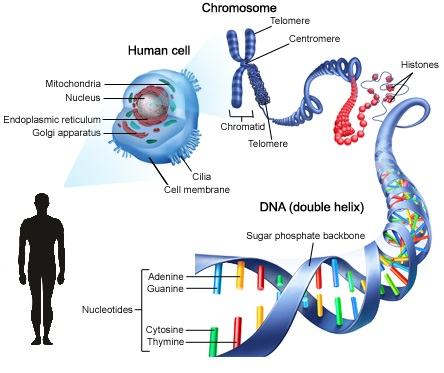
\includegraphics[width=9.5cm]{./humanToCell}
\end{center}
\end{frame}
 
\begin{frame}
	\frametitle{Mutation}
	\begin{figure}
		\centering
		\tikzstyle{block} = [rectangle, draw, line width=0.5mm,
		text centered]
		\tikzstyle{line} = [draw, -latex']
		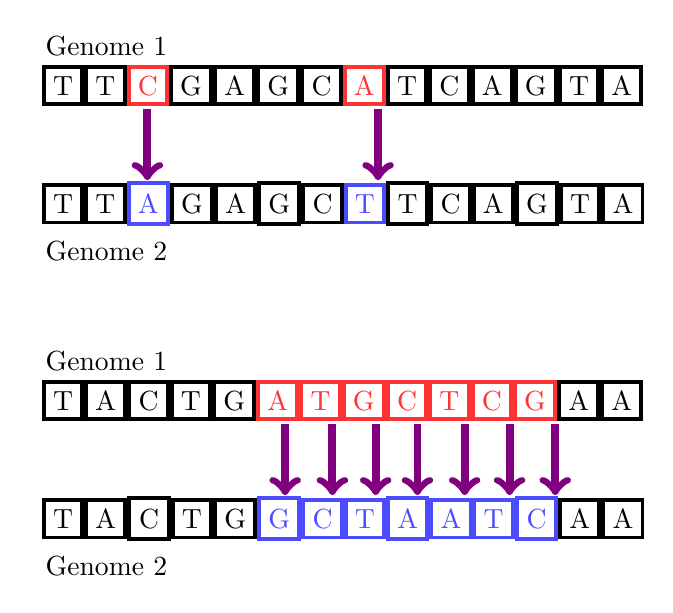
\begin{tikzpicture}[auto, node distance = 5mm]
		%Reference
		\node [rectangle, minimum width=2cm](lab) at (4.05,0) {Genome 1};
		\node [block, below of=lab] (Val1_2) at (3.5,0) {T};
		\node [block, anchor=west] (Val1_3) at (Val1_2.east) {T};
		\node [block, anchor=west, color=red!80] (Val1_4) at (Val1_3.east) {C};
		\node [block, anchor=west] (Val1_5) at (Val1_4.east) {G};
		\node [block, anchor=west] (Val1_6) at (Val1_5.east) {A};
		\node [block, anchor=west] (Val1_7) at (Val1_6.east) {G};
		\node [block, anchor=west] (Val1_8) at (Val1_7.east) {C};
		\node [block, anchor=west, color=red!80] (Val1_9) at (Val1_8.east) {A};
		\node [block, anchor=west] (Val1_10) at (Val1_9.east) {T};
		\node [block, anchor=west] (Val1_11) at (Val1_10.east) {C};
		\node [block, anchor=west] (Val1_12) at (Val1_11.east) {A};
		\node [block, anchor=west] (Val1_13) at (Val1_12.east) {G};
		\node [block, anchor=west] (Val1_14) at (Val1_13.east) {T};
		\node [block, anchor=west] (Val1_15) at (Val1_14.east) {A};
		
		\node [rectangle, minimum width=2cm](lab2) at (4.05,-2.6) {Genome 2};
		%second line
		\node [block] (Val2_2) at (3.5,-2) {T};
		\node [block, anchor=west] (Val2_3) at (Val2_2.east) {T};
		\node [block, anchor=west, color=blue!70,minimum height=5.2mm, minimum width=5mm] (Val2_4) at (Val2_3.east) {A};
		\node [block, anchor=west] (Val2_5) at (Val2_4.east) {G};
		\node [block, anchor=west] (Val2_6) at (Val2_5.east) {A};
		\node [block, anchor=west,minimum height=5.2mm, minimum width=5mm] (Val2_7) at (Val2_6.east) {G};
		\node [block, anchor=west] (Val2_8) at (Val2_7.east) {C};
		\node [block, color=blue!70, anchor=west] (Val2_9) at (Val2_8.east) {T};
		\node [block, anchor=west,minimum height=5.2mm, minimum width=5mm] (Val2_10) at (Val2_9.east) {T};
		\node [block, anchor=west] (Val2_11) at (Val2_10.east) {C};
		\node [block, anchor=west] (Val2_12) at (Val2_11.east) {A};
		\node [block, anchor=west,minimum height=5.2mm, minimum width=5mm] (Val2_13) at (Val2_12.east) {G};
		\node [block, anchor=west] (Val2_14) at (Val2_13.east) {T};
		\node [block, anchor=west] (Val2_15) at (Val2_14.east) {A};
		
		%arrows
		\draw[line width=1mm,color=red!50!blue,->] (4.57,-0.8) -- (4.57,-1.7);
		%\draw[line width=1mm,color=black!70,->] (6.32,-0.8) -- (6.32,-1.7);
		%\draw[line width=1mm,color=blue!50,->] (8,-0.8) -- (8,-1.7);
		\draw[line width=1mm,color=red!50!blue,->] (7.5,-0.8) -- (7.5,-1.7);
		
		%Reverse Complement of Reference
		\node [rectangle, minimum width=2cm](lab3) at (4.05,-4) {Genome 1};
		\node [block, below of=lab3] (Val3_2) at (3.5,-4) {T};
		\node [block, anchor=west] (Val1_3) at (Val3_2.east) {A};
		\node [block, anchor=west] (Val1_4) at (Val1_3.east) {C};
		\node [block, anchor=west] (Val1_5) at (Val1_4.east) {T};
		\node [block, anchor=west] (Val1_6) at (Val1_5.east) {G};
		\node [block, anchor=west, color=red!80] (Val1_7) at (Val1_6.east) {A};
		\node [block, anchor=west, color=red!80] (Val1_8) at (Val1_7.east) {T};
		\node [block, anchor=west, color=red!80] (Val1_9) at (Val1_8.east) {G};
		\node [block, anchor=west, color=red!80] (Val1_10) at (Val1_9.east) {C};
		\node [block, anchor=west, color=red!80] (Val1_11) at (Val1_10.east) {T};
		\node [block, anchor=west, color=red!80] (Val1_12) at (Val1_11.east) {C};
		\node [block, anchor=west, color=red!80] (Val1_13) at (Val1_12.east) {G};
		\node [block, anchor=west] (Val1_14) at (Val1_13.east) {A};
		\node [block, anchor=west] (Val1_15) at (Val1_14.east) {A};
		%gapped reverse complement
		\node [rectangle, minimum width=2cm](lab4) at (4.05,-6.6) {Genome 2};
		
		\node [block] (Val4_2) at (3.5,-6) {T};
		\node [block, anchor=west] (Val2_3) at (Val4_2.east) {A};
		\node [block, anchor=west, minimum height=5.2mm, minimum width=5mm] (Val2_4) at (Val2_3.east) {C};
		\node [block, anchor=west] (Val2_5) at (Val2_4.east) {T};
		\node [block, anchor=west] (Val2_6) at (Val2_5.east) {G};
		\node [block, color=blue!70, anchor=west, minimum height=5.2mm, minimum width=5mm] (Val2_7) at (Val2_6.east) {G};
		\node [block, color=blue!70, anchor=west] (Val2_8) at (Val2_7.east) {C};
		\node [block, color=blue!70, anchor=west] (Val2_9) at (Val2_8.east) {T};
		\node [block, color=blue!70, anchor=west, minimum height=5.2mm, minimum width=5mm] (Val2_10) at (Val2_9.east) {A};
		\node [block, color=blue!70, anchor=west] (Val2_11) at (Val2_10.east) {A};
		\node [block, color=blue!70, anchor=west] (Val2_12) at (Val2_11.east) {T};
		\node [block, color=blue!70, anchor=west, minimum height=5.2mm, minimum width=5mm] (Val2_13) at (Val2_12.east) {C};
		\node [block, anchor=west] (Val2_14) at (Val2_13.east) {A};
		\node [block, anchor=west] (Val2_15) at (Val2_14.east) {A};
		
		%arrows
		\draw[line width=1mm,color=red!50!blue,->] (6.32,-4.8) -- (6.32,-5.7);
		\draw[line width=1mm,color=red!50!blue,->] (6.92,-4.8) -- (6.92,-5.7);
		\draw[line width=1mm,color=red!50!blue,->] (7.47,-4.8) -- (7.47,-5.7);
		\draw[line width=1mm,color=red!50!blue,->] (8,-4.8) -- (8,-5.7);
		\draw[line width=1mm,color=red!50!blue,->] (8.6,-4.8) -- (8.6,-5.7);
		\draw[line width=1mm,color=red!50!blue,->] (9.17,-4.8) -- (9.17,-5.7);
		\draw[line width=1mm,color=red!50!blue,->] (9.75,-4.8) -- (9.75,-5.7);
		
		\end{tikzpicture}
		\caption{Random mutations and Segment mutation.}
	\end{figure}
\end{frame}

\begin{frame}
	\frametitle{Mapper}
	\begin{figure}
		\centering
		
		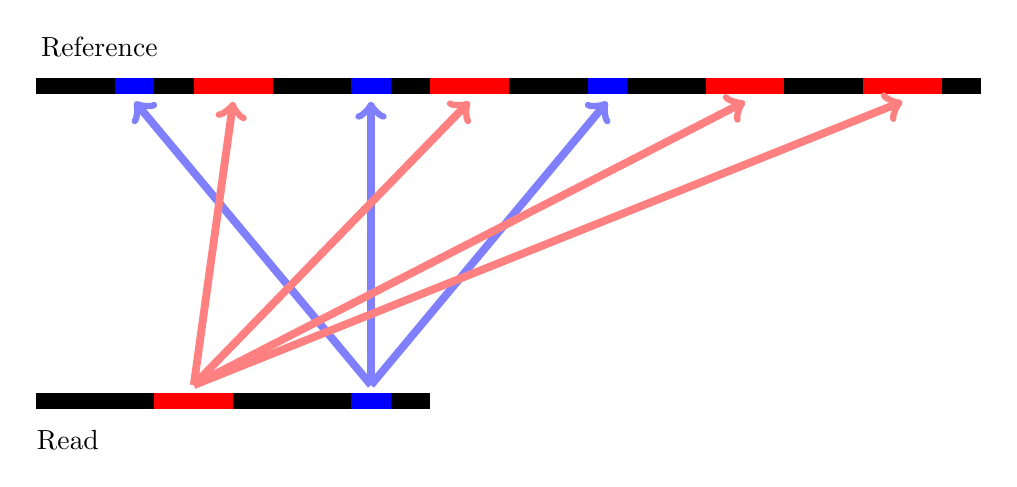
\begin{tikzpicture}[]
		
		%reference
		\draw[line width=2mm] (0,4) -- (12,4);
		\draw[line width=2mm,color=red] (2,4) -- (3,4);
		\draw[line width=2mm,color=red] (10.5,4) -- (11.5,4);
		\draw[line width=2mm,color=red] (8.5,4) -- (9.5,4);
		\draw[line width=2mm,color=red] (5,4) -- (6,4);
		\draw[line width=2mm,color=blue] (7,4) -- (7.5,4);
		\draw[line width=2mm,color=blue] (1,4) -- (1.5,4);
		\draw[line width=2mm,color=blue] (4,4) -- (4.5,4);
		%read
		\draw[line width=2mm] (0,0) -- (5,0);
		\draw[line width=2mm,color=red] (1.5,0) -- (2.5,0);
		\draw[line width=2mm,color=blue] (4,0) -- (4.5,0);
		%labels
		\node[rectangle](refer) at (0.8,4.5) {Reference};
		
		\node[rectangle](refer) at (0.4,-0.5) {Read};
		%arrows
		\draw[line width=1mm,color=blue!50,->] (4.25,0.2) -- (1.25,3.8);
		\draw[line width=1mm,color=blue!50,->] (4.25,0.2) -- (7.25,3.8);
		\draw[line width=1mm,color=blue!50,->] (4.25,0.2) -- (4.25,3.8);
		\draw[line width=1mm,color=red!50,->] (2,0.2) -- (2.5,3.8);
		\draw[line width=1mm,color=red!50,->] (2,0.2) -- (11,3.8);
		\draw[line width=1mm,color=red!50,->] (2,0.2) -- (9,3.8);
		\draw[line width=1mm,color=red!50,->] (2,0.2) -- (5.5,3.8);
		\end{tikzpicture}
		\caption{Mapping is just indicating the clusters of a large segment of the read in reference.} 
	\end{figure}
\end{frame}

\begin{frame}
	\frametitle{Aligner}
	\begin{figure}
		\centering
		
		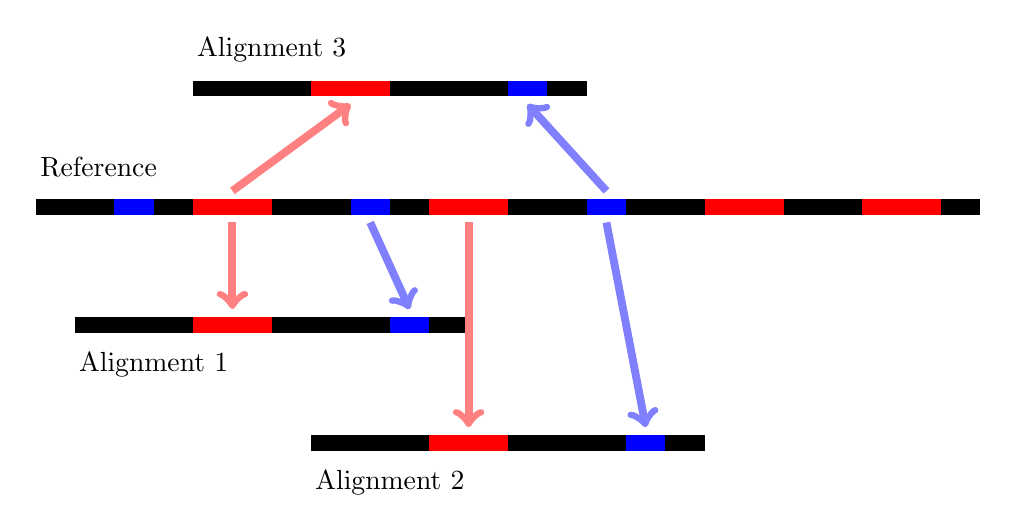
\begin{tikzpicture}[]
		
		%reference
		\draw[line width=2mm] (0,3) -- (12,3);
		\draw[line width=2mm,color=red] (2,3) -- (3,3);
		\draw[line width=2mm,color=red] (10.5,3) -- (11.5,3);
		\draw[line width=2mm,color=red] (8.5,3) -- (9.5,3);
		\draw[line width=2mm,color=red] (5,3) -- (6,3);
		\draw[line width=2mm,color=blue] (7,3) -- (7.5,3);
		\draw[line width=2mm,color=blue] (1,3) -- (1.5,3);
		\draw[line width=2mm,color=blue] (4,3) -- (4.5,3);
		%read 1
		\draw[line width=2mm] (0.5,1.5) -- (5.5,1.5);
		\draw[line width=2mm,color=red] (2,1.5) -- (3,1.5);
		\draw[line width=2mm,color=blue] (4.5,1.5) -- (5,1.5);
		%read 2
		\draw[line width=2mm] (3.5,0) -- (8.5,0);
		\draw[line width=2mm,color=red] (5,0) -- (6,0);
		\draw[line width=2mm,color=blue] (7.5,0) -- (8,0);
		%read 3
		\draw[line width=2mm] (2,4.5) -- (7,4.5);
		\draw[line width=2mm,color=red] (3.5,4.5) -- (4.5,4.5);
		\draw[line width=2mm,color=blue] (6,4.5) -- (6.5,4.5);
		%labels
		\node[rectangle](refer) at (0.8,3.5) {Reference};
		\node[rectangle](refer) at (1.5,1) {Alignment 1};
		\node[rectangle](refer) at (4.5,-0.5) {Alignment 2};
		\node[rectangle](refer) at (3,5) {Alignment 3};
		%arrows
		\draw[line width=1mm,color=red!50,->] (5.5,2.8) -- (5.5,0.2);
		\draw[line width=1mm,color=blue!50,->] (7.25,2.8) -- (7.75,0.2);
		\draw[line width=1mm,color=red!50,->] (2.5,2.8) -- (2.5,1.7);
		\draw[line width=1mm,color=blue!50,->] (4.25,2.8) -- (4.75,1.7);
		\draw[line width=1mm,color=red!50,->] (2.5,3.2) -- (4,4.3);
		\draw[line width=1mm,color=blue!50,->] (7.25,3.2) -- (6.25,4.3);
		\end{tikzpicture}
		\caption{Three possible alignments based on the read mapping.} 
	\end{figure}
\end{frame}